\subsection{Data From \gls{smc}}
Above in \cref{sec:queries} we discussed different queries relevant for collecting data from the schedule, here we will illustrate what this data may look like, and discuss the usefulness thereof. We will in particular focus on the queries with keyword \textit{simulate}, as they are included for the purpose of extracting data. Despite of it being described we will run $100$ simulations of these queries, for the purpose of this section fewer will be run in order to visualise the data. 

\begin{figure}[h]
	\centering
	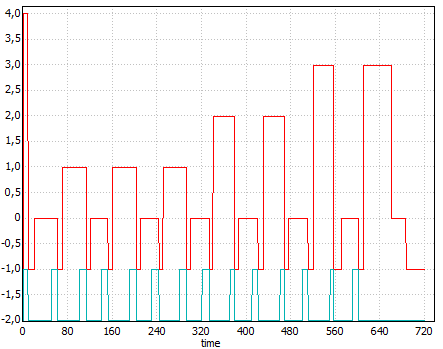
\includegraphics[scale=0.8]{graphics/active_running.png}
	\caption{Result of running query \ref{eq:smc4} in the UPPAAL GUI}
	\label{fig:active_running}
\end{figure}

First consider query \cref{eq:smc4}, this will result in a graph showing what payloads was supposed to run when and whether or not they were so. We have run this query through the UPPAAL GUI and resulting the graph seen in \cref{fig:active_running}. It should be noted that such graphs are not made available to the user via our system, but all the values needed to make such a graph is saved and made available to the user.

We can in \cref{fig:active_running} see that all payloads are executed except for the last two. This can be seen by looking at the parts where the red curve is different from $-1$, if the blue curve at any time in this period differs from $-2$ it means the payload was executed. \\
The reason for the last two not being executed, is that executing them would result in depletion of the available well, as can be seen in \cref{fig:sim5a} on the left. 

\begin{figure}[h]%
	\centering
	\subfloat
	{{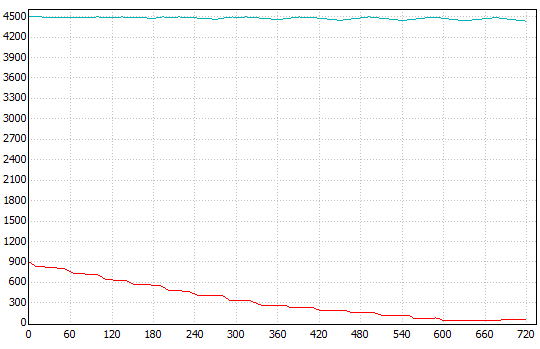
\includegraphics[width=7cm,,clip] {graphics/simAB1.png} }}%
	\qquad
	\subfloat
	{{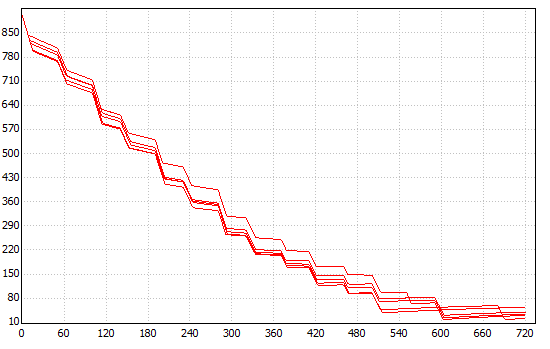
\includegraphics[width=7cm,clip] {graphics/sim5A.png} }}%
	\caption{1 simulation of \textit{a} and \textit{b}(left) 5 simulations of \textit{a}(right)}%
	\label{fig:sim5a}%
\end{figure}

On the left in \cref{fig:sim5a} we see the battery wells available(red), and bound(blue) over one simulation, for this example the starting capacity in the wells are $900$ in the available and $4500$ in the bound well. It can be seen that the bound well is relatively stable, meaning its capacity does not vary much, whereas the available well gets close to depletion, resulting in the last two payloads in \cref{fig:active_running} being skipped. \\
In \cref{fig:sim5a} on the right the available well, \uppVar{a}, have been simulated five times. This shows some interesting results, for some of the simulations the same skips occur as in \cref{fig:active_running}, the last two, whereas some simulations result in the very last payload being executed but the two prior to it being skipped. This is a result of execution time of payloads may vary, and thus consume more power, in the \gls{smc} model.